\documentclass{beamer}
\usepackage{graphicx}
\usepackage{color}
%\graphicspath{{}}

\title{Data Mining Hospital Readmissions and Mortality Rates using Multiagent Random Forest}
\author{Andrew Berry}
\begin{document}
	\frame{\titlepage}
	\begin{frame}
		\frametitle{Introduction}
		% A very brief overview of your project concept and the DAI question you are addressing
		\begin{itemize}
			\item Goal: Attempt to accurately predict location of hospital based on readmissions and death metrics
			\item Subgoal: Establish that there exists a correlation between such metrics and location
			\item Subgoal: Attempt to improve prediction accuracy by introducing multiagent communication
		\end{itemize}
	\end{frame}

	\begin{frame}
		\frametitle{System Description}
		\begin{itemize}
			\item Dataset: Hospital Readmission and Death Rates of US Hospitals
			\item Data analysis (dataframe manipulation): Pandas
			\item Machine Learning: Scikit-Learn
			\item Multiagent system: SPADE
		\end{itemize}
	\end{frame}

	\begin{frame}
		\frametitle{System Description}
		\begin{itemize}
			\item Initial agent network:
			%TODO insert graphic
		\end{itemize}
	\end{frame}

	\begin{frame}
		\frametitle{System Description}
		\begin{itemize}
			\item Final agent network:
			%TODO insert graphic
		\end{itemize}
	\end{frame}

	\begin{frame}
		\frametitle{Experiment 1}
		\begin{itemize}
			\item $n = 30$
			\item $t = 100$
			\item $\mu = gini$
		\end{itemize}
		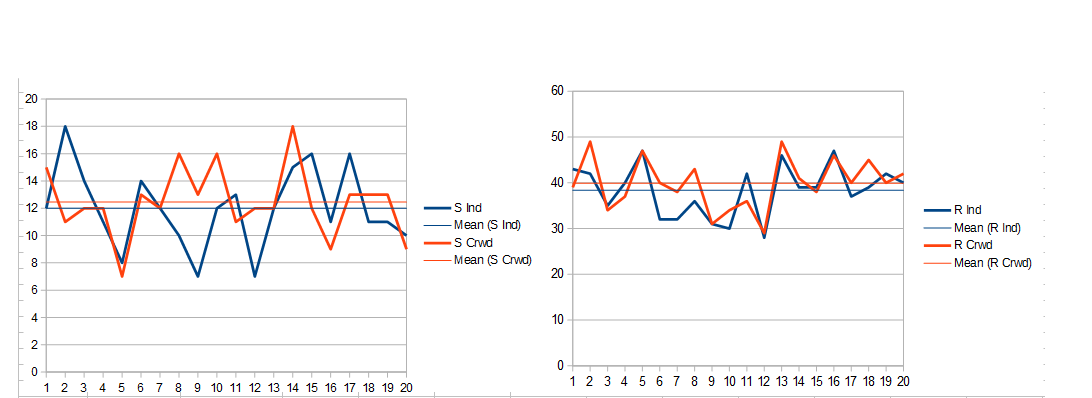
\includegraphics[width=11cm, height=5cm]{e1_comparative}
	\end{frame}

	\begin{frame}
		\frametitle{Experiment 1}
		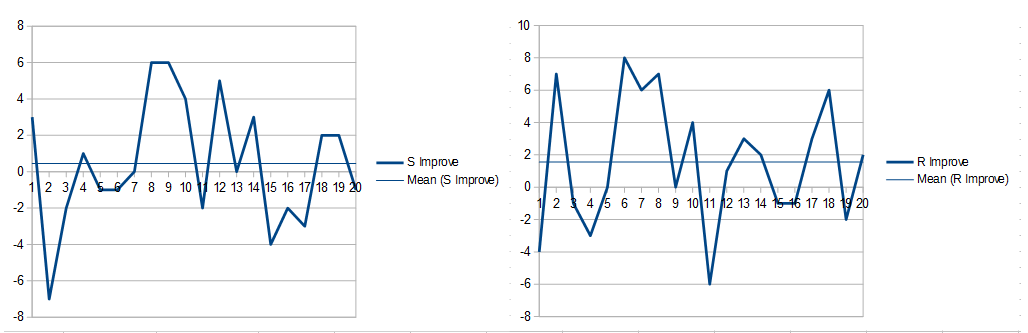
\includegraphics[width=11cm, height=5cm]{e1_improvement}
	\end{frame}

	\begin{frame}
		\frametitle{Experiment 2}
		\begin{itemize}
			\item $n = 10$
			\item $t = 100$
			\item $\mu = entropy$
		\end{itemize}
		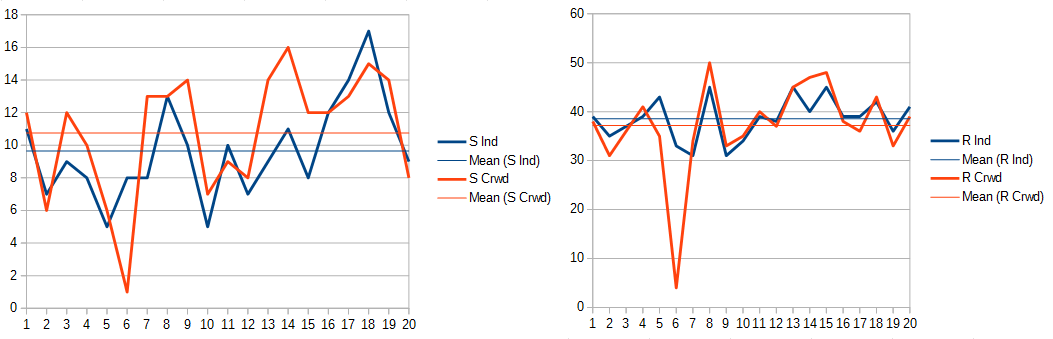
\includegraphics[width=11cm, height=5cm]{e2_comparative}
	\end{frame}

	\begin{frame}
		\frametitle{Experiment 2}
		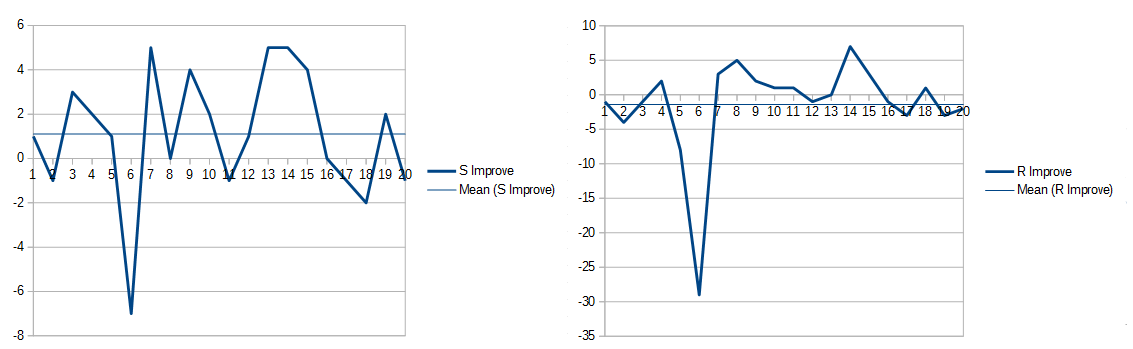
\includegraphics[width=11cm, height=5cm]{e2_improvement}
	\end{frame}

	\begin{frame}
		\frametitle{Demo}
	\end{frame}

	\begin{frame}
		\frametitle{Conclusions}
		\begin{itemize}
			\item Correlation is apparent
			\item Improvement from multiagent system fairly uncertain
		\end{itemize}
	\end{frame}

%	\begin{frame}
%		\frametitle{Contribution 1: Game Abstraction Framework}
%		\begin{itemize}
%			\item Previous research deals with opportunistic crime, but fails to scale
%			\item This paper uses abstraction to address this
%			\item Abstract layer generated from original 
%				\begin{itemize}
%					\item Contains aggregated targets (aggregated from similar targets in original)
%				\end{itemize}
%		\end{itemize}
%		\includegraphics[width=3cm, height=5cm]{abstraction}
%	\end{frame}
%
%	\begin{frame}
%		\frametitle{Questions?}
%		%{\huge {\color{blue} Questions?}}
%	\end{frame}

\end{document}
